%========================%
%        Preamble        %
%========================%
\documentclass[12pt]{amsart}

    %========================%
%        Packages        %
%========================%

\usepackage[utf8]{inputenc}
%\usepackage{amsmath}    % Included in amsart package
%\usepackage{amsthm}     % 
\usepackage{amssymb}      % 
\usepackage{mathtools}      % Paired Limiter Macros
% \usepackage{mdframed}       % boxes for theorem
\usepackage{enumitem}     % Continuous numbering of lists
\usepackage[hidelinks]{hyperref}
\usepackage{tikz}
\usetikzlibrary{positioning}
\usepackage{blindtext}
\usepackage{graphicx}
\usepackage{float}

%========================% 
%          Title         %
%========================% 
\title{Lecture 1 and 2}
\author{Anish Sundaram}
\date{\today}

%========================% 
%        Theorems        %
%========================% 
\theoremstyle{definition}
\newtheorem{theorem}{Theorem}  % Boxed theorems
\newtheorem{definition}{Definition} % Definitions
\newtheorem{example}{Example}       %
\newtheorem{algorithm}{Algorithm}
\newtheorem*{proof*}{Proof}         % non-numbered
\newtheorem*{remark}{Remark}        %
\numberwithin{equation}{theorem}    % Local equation numbering

\setcounter{tocdepth}{3}      % Show subsubsections in contents

%========================% 
%        Macros          %
%========================% 
\DeclarePairedDelimiter\abs{\lvert}{\rvert}  % Vertical bars
\DeclarePairedDelimiter\norm{\lVert}{\rVert} % Double vertical bars
\newcommand{\drawvec}[1]{                    % matrices on one line
    \begin{bmatrix}
        #1
    \end{bmatrix}
}


% \begin{figure}[H]
%     \centering
%     \includegraphics[width=5in]{global-carbon-cycle.png}
%     \caption{The Global Carbon Cycle}
%     \label{global-carbon-cycle}
% \end{figure}

%========================% 
%         Document       %
%========================% 
\begin{document}

\maketitle

\tableofcontents

\section*{1 Populations Samples and Descriptive Statistics}

\subsection*{1.1 What are Statistics}
\begin{definition}
    \textbf{Uncertainty}:
    Whenever data are involved, there is almost always uncertainty (aka randomness, stochasticity, error, etc). Data sets are invariably measured with some error.
\end{definition}

\begin{definition}
    \textbf{Statistics}:
    Statistics is the practice  collecting and analyzing numerical data in large quantities, especially for the purpose of inferring proportions in a whole from those in a representative sample.
\end{definition}

\subsection*{1.2 Population and Sampling}
\begin{definition}
    \textbf{Population(N)}:
    The entire group of objects {$W_1 ....W_N$}
    \begin{remark}
        Typically the size of Population N is very large, or its result isnt very meaningful
    \end{remark}
\end{definition}

\begin{definition}
    \textbf{Sample(n)}:
    Samples are sub-sections of the populations where typically we look at different cross-sections of the population
\end{definition}

\begin{definition}
    \textbf{Population Mean/Average($\mu$)}:
    $$\mu = \frac{1}{N} \sum _{i=1}^{N} w_i = \frac{w_1 + w_2 +w_N}{N}$$
\end{definition}

\begin{definition}
    \textbf{Sample Mean($\bar{x}$)}:
    Sample mean is the arithmetic average of the measurements in the sample, found mathematically by:
    $$\bar{X_n} =\frac{1}{n} \sum _{i=1}^{n} = \frac{X_1 + X_2 +X_n}{n}$$
    \begin{remark}
        Naturally,$\bar{X_n}$ a “very good” approximation of the $\mu$ especially forlarge sample sizes n.
    \end{remark}
\end{definition}

\subsection*{1.3 Sampling Error}

\begin{definition}
    \textbf{Statistic}:
    A quanitity based on a smaple and meant to estiamate a population parameter
    \begin{remark}
        The sample mean$X_n$ is a statistic used to estmate the pipulation parameter $\mu$
    \end{remark}
\end{definition}

\subsection*{1.4 Random Sampling}

\begin{definition}
    \textbf{Simple Random Sampling(SRS)}:
    Random sampling is a part of the sampling technique in which each sample has an equal probability of being chosen. A sample chosen randomly is meant to be an unbiased representation of the total population.

    \begin{remark}
        Simple Random Sampling is the hallmark of collecting representative samples from the population. 
    \end{remark}
\end{definition}

\begin{definition}
    \textbf{Double-blinded Randomized Trials}:
    A randomized trial in which the subjects are divided into two groups, one with the treatment and one with a placebo, and neither the doctor handing treatment nor the patient know which pill is which, only the directors.
\end{definition}

\subsection*{1.5 Other types of Sampling}

\begin{definition}
    \textbf{Convenience Sampling}:
    Random samples may be impossible to come by and sometimes researchers settle at convenience sampling, sampling groups that may not be representative and pigeonholed yet easy to test. This is prone to \textbf{Selection Bias}
\end{definition}

\begin{definition}
    \textbf{Voluntary Sampling}:
    Samples where people voluteer themselves to be included into the study because only those with a strong opinion will respond which will polarize results. This is also prone to \textbf{Selection Bias}
\end{definition}

\begin{definition}
    \textbf{Stratified Sampling}:
    A method of sampling where we divide the population into homogeneous subgroups before doing an SRS. 
\end{definition}

\subsection*{1.6 Types of Data}

\begin{definition}
    \textbf{Types of Data}:
    \begin{enumerate}
        \item \textbf{Categorical Data}:
        Non-numerical values such as gender, blood type, ethnicity. Essentially char-based types 
        \item \textbf{Numerical Data}:
        Real number values on a continuous interval, for example temperature, weight, insurance losses, concentration, etc. Ints or Floats
        \item \textbf{Ordinal/Count Data}:
        Typically, non-negative integer-valued data, e.g.,number of accidents on I-95 during the period of a week; number of foxes in a given area; number of gamma-ray bursts.
    \end{enumerate}
\end{definition}

\subsection*{1.7 Measures of Location}

\begin{definition}
    \textbf{Outliers}:
    Numerical Values much smaller or much smaller the average selection of values. Outliers can skew measurements which are sensitive to outliers like the Mean and can render them inappropriate.
\end{definition}

\begin{definition}
    \textbf{Linearity}:
    The ability of a set of data to be fit by a linear regression line. The mean is a linear function of the data.
\end{definition}

\begin{definition}
    \textbf{Median}:
    The Median is the literal middle value of a dataset, and is calculated the same way. The Median is robust to outliers such that outliers are not impactful.
\end{definition}

\subsection*{1.8 Measures of Variability}
\begin{definition}
    \textbf{Population Standard Deviation($\sigma$)}:
    Standard Deviation is a quantity calculated to indicate the extent of deviation for a group as a whole. It can be mathematically found by the equation: 
    $$\sigma = \sqrt{\frac{1}{N}\sum^{N}_{i=1}(w_1 - \mu)^2}$$ for a population
\end{definition}

\begin{definition}
    \textbf{Population Variance($\sigma^2$)}:
    Variance qualifies how dispersed the data is from the mean $\mu$ and is calculated as the square of the Standard Deviation $\sigma$ in order to get a positive distance value and to amplify the effect.
\end{definition}

\begin{definition}
    \textbf{Sample Standard Deviation and Variance($s$ and $s^2$)}:
    For samples the formula for finding the standard deviation and resulting variance are linked but use sample values as opposed to population parameters:
    $$s = \sqrt{\frac{1}{n-1}\sum^{n}_{i=1}(X_1 - \bar{X_n})^2}$$ and the variance($s^2$) is simply the square.
\end{definition}
 
\subsection*{1.9 Chebyshev's Inequality}
\begin{theorem}
    \textit{Chebyshev's Inequality}:
        The proportion of the population values farther than k>1 standard deviations($\sigma$) from the mean $\mu$ is no greater than $1 - \frac{1}{k^2}$.
\end{theorem}

\section*{2 More on descriptive and Graphical Statistcs}

\subsection*{2.1 Stem-and-leaf and Dot plots}

\begin{definition}
    
    \textbf{Stem-and-leaf Plot}:
    Graph consisting of a stem a which contains a shared point, and various leafs which all "branch from the stem". For example: 
    \begin{enumerate}
        \item 4 | 259 
        \item 5 | 0111133556678
        \item 6 | 067789
        \item 7 | 0123344456666699
        \item 8 | 000012223344456668
        \item 9 | 013
    \end{enumerate} 
\end{definition}

\begin{definition}
    \textbf{Dot-plots}:
    Useful for small to moderate data sets the dot plot involves placing stacked dots to represent number of times a value has been reached per value apparent. Very similar to Histograms
\end{definition}


\begin{figure}[H]
    \centering
    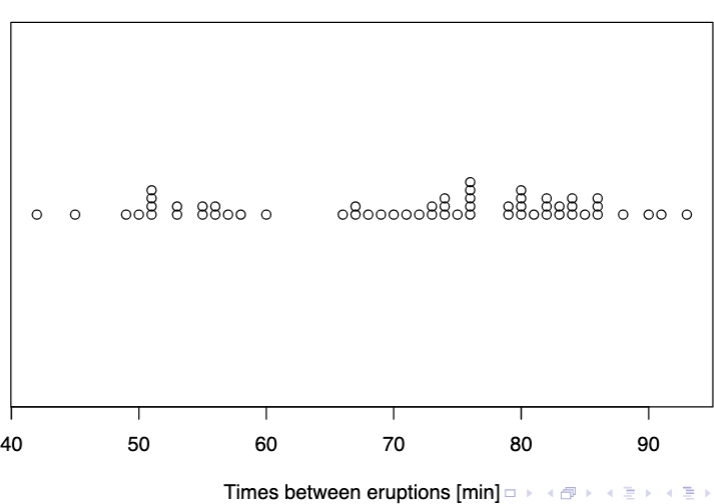
\includegraphics[width=3in]{Media/dotplot.png}
    \caption{Example of a Dotplot}
    \label{Dotplot}
\end{figure}

\subsection*{2.2 Histograms}

\begin{definition}
    \textbf{Histogram}:
    Similar to dot-plots but using buckets for value ranges as opposed to including every single point value, essentially an abstraction of a dot-plot.
    Bins are arranged [x,y) aside from the last bin which is [x,y]
\end{definition}

\begin{definition}
    \textbf{Relative Frequency Graph}:
    A relative frequency histogram is a type of graph that shows how often something happens, in percentages. Essentially we relate how much of the total sample rests within each bin using the equation $$R_i = \frac{F_i}{N}$$
\end{definition}


\begin{figure}[H]
    \centering
    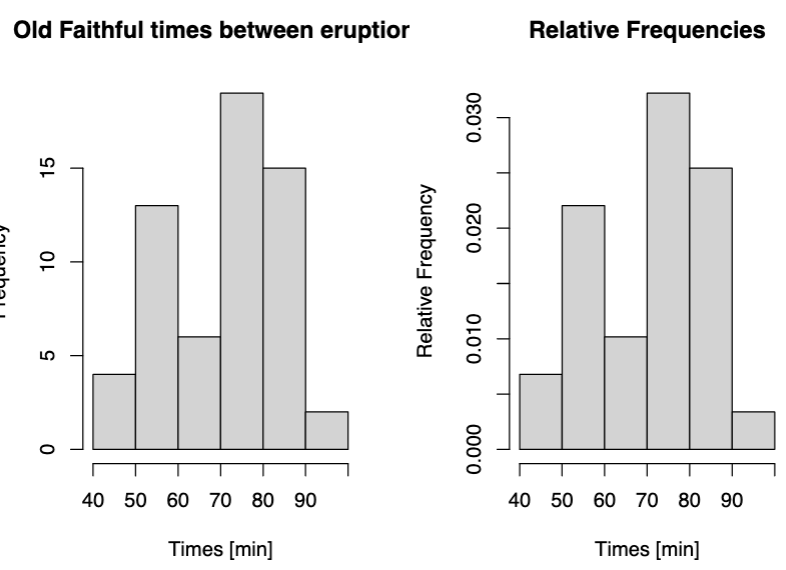
\includegraphics[width=3in]{Media/histogram.png}
    \caption{Example of  Histogram}
    \label{Histogram}
\end{figure}

\begin{theorem}
    \textit{Friedman-Diaconis rule}:
    A method of determining how many bins k or the bin-size. $$k \approx \frac{range}{2 \cdot IQR} \cdot N^{1/3}$$
\end{theorem}

\subsection*{2.3 Box-plots}
\begin{definition}
    \textbf{Inter-Quartile Range(IQR)}:
    The difference between the 3rd and 1st quartiles in a dataset, in other words the middle 50 percent. The IQR is a measure of variability and can be found by:
    $$IQR = q(0.75)- q(0.25)$$
\end{definition}

\begin{definition}
    \textbf{Box-plots}:
    A easy-to-grasp visual summary of location, variability, and outliers using quartiles and outlier points. The box itself is constructed from the 1st and 3rd quartiles with a line at the median, and whiskers indicating the most extreme values within 1.5 * IQR from the nearest quartile.
    \begin{remark}
        The outliers are all observations farther than 1.5×IRQ from thenearest quartile – they are all displayed as circles.
    \end{remark}
\end{definition}

\begin{figure}[H]
    \centering
    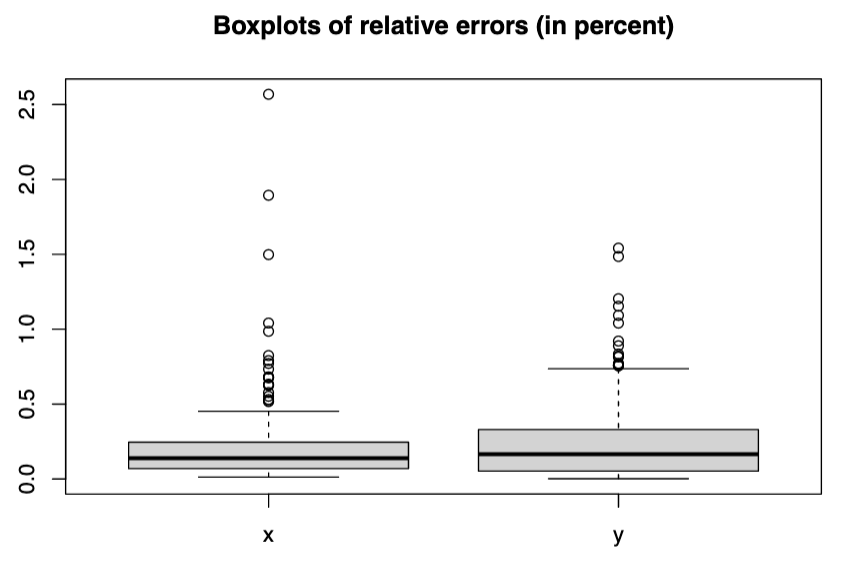
\includegraphics[width=3in]{Media/Boxplot.png}
    \caption{Example of a Boxplot}
    \label{Boxplot}
\end{figure}

\end{document}